\documentclass[aspectratio=1610,xcolor=dvipsnames,table]{beamer}


\xdefinecolor{darkgreen}{RGB}{000, 88, 000}
\xdefinecolor{greyblue}{RGB}{200, 200, 255}
\makeatletter
\newcommand*{\mylength}[1]{\strip@pt#1}
% Or rounded back to `cm` (there will be some rounding errors!)
%\newcommand*{\getlength}[1]{\strip@pt\dimexpr0.035146\dimexpr#1\relax\relax}

\makeatother

\mode<presentation>
{
  \usetheme{Luebeck}
%\usecolortheme[named=PineGreen]{structure}
\usecolortheme[named=gray]{structure}
  \setbeamercovered{invisible}
\setbeamertemplate{mini frames}[box]
\setbeamertemplate{navigation symbols}{}}


\setbeamercolor{block title example}{bg=blue,fg=white}%bg=background, fg= foreground
\setbeamercolor{block body example}{bg=structure.bg!90!blue,fg=black}%bg=background, fg= foreground

%\usepackage{pifont}
\usepackage{ulem}
\usepackage{epstopdf}
\usepackage{wasysym}

\setcounter{tocdepth}{1}


%\useinnertheme{rectangles}
\useoutertheme{infolines}

%\loadgraphics{logo-pi-bunt3,lhcb-logo,unisiegel-gray}
\newsavebox{\unilogo} \newsavebox{\pilogo} \newsavebox{\lhcblogo}
\sbox{\unilogo}{\raisebox{0.5mm}{\hspace{0.5mm}
\includegraphics[height=1.15cm]{../pics/unihei_logo_red}}}
%\sbox{\pilogo}{\includegraphics[height=1.25cm]{logo-pi-bunt3}}
\sbox{\pilogo}{
\includegraphics[height=1.25cm]{../pics/logo-pi-bunt}}
\sbox{\lhcblogo}{
\includegraphics[height=1.25cm]{../pics/lhcb-logo}}

\setbeamertemplate{footline}
{
  \leavevmode%
  \hbox{%
  \begin{beamercolorbox}[wd=.333333\paperwidth,ht=2.25ex,dp=1ex,left]{author in head/foot}%
    \usebeamerfont{author in head/foot}\vtop{\vskip-2.25ex\hbox{\resizebox{!}{3.25ex}{\usebox{\pilogo}}}}%
    \hfill \insertshortauthor~~(\insertshortinstitute) \hfill%
  \end{beamercolorbox}%
  \begin{beamercolorbox}[wd=.333333\paperwidth,ht=2.25ex,dp=1ex,center]{title in head/foot}%
    \usebeamerfont{title in head/foot}\insertshorttitle%
  \end{beamercolorbox}%
  \begin{beamercolorbox}[wd=.333333\paperwidth,ht=2.25ex,dp=1ex,right]{date in head/foot}%
    \usebeamerfont{date in head/foot}\insertshortdate{}\hspace*{2em}%
    \insertframenumber{} / \inserttotalframenumber\hspace*{2ex} \vtop{\vskip-2.25ex\hbox{\resizebox{!}{3.25ex}{\usebox{\lhcblogo}}}}%
  \end{beamercolorbox}}%
  \vskip0pt%
}

\setbeamertemplate{frametitle}
{
  \ifbeamercolorempty[bg]{frametitle}{}{\nointerlineskip}%
  \leavevmode%
  \vskip-2pt\hbox{%
  \begin{beamercolorbox}[wd=\paperwidth,left]{frametitle}%
    \usebeamerfont{frametitle}%
    \vskip.125ex%
    \hbox{\vtop{\raisebox{-1ex}[1ex][1ex]{\makebox[0pt][l]{\usebox{\unilogo}}}%
    \hspace{1.5cm}\strut\insertframetitle\strut}\par%
    {%
      \ifx\insertframesubtitle\@empty%
      \else%
      {\usebeamerfont{framesubtitle}\usebeamercolor[fg]{framesubtitle}\insertframesubtitle\strut\par}%
      \fi
    }}%
  \end{beamercolorbox}%
  }%
}


\usepackage[english]{babel}
\usepackage[utf8]{inputenc}
\usepackage{graphicx}
\DeclareGraphicsRule{*}{mps}{*}{}
\usepackage[absolute,overlay]{textpos}
\setlength{\TPHorizModule}{10mm}
\setlength{\TPVertModule}{\TPHorizModule}
\textblockorigin{0mm}{13mm} % start everything near the top-left                                                                                                                                                                                              % corner                   
\usepackage{pgf}
\usepackage{times}
\usepackage[T1]{fontenc}

\usepackage[math]{iwona}

\usepackage[mathscr]{eucal}
\usepackage{mathrsfs}
\usepackage{amsfonts}
\usepackage{amsmath} %,abhepexpt,abhep}
\usepackage{amssymb}

\usepackage{fontspec}
\setmainfont{Montserrat-Regular}
%\setsansfont[BoldFont={Montserrat-Bold}, Ligatures=TeX]{Montserrat-Regular}


\usepackage{verbatim}
% \usepackage[amssymb]{SIunits}
%\usepackage{natbib}

\usepackage{hepparticles}
\usepackage{hepnicenames}
\usepackage{hepunits}
\usepackage{tikz}
%\usetikzlibrary{trees}
%\usetikzlibrary{decorations.pathmorphing}
%\usetikzlibrary{decorations.markings}
\usetikzlibrary{arrows}
\usetikzlibrary{shapes}
%\usetikzlibrary{positioning}
%\usetikzlibrary{patterns}
%\usetikzlibrary{fit}
%\usepackage{verbatim}
\usepackage{multicol}
\usepackage{colortbl} 
\usepackage{multirow}
\usepackage{ragged2e}
\usepackage{listings}

%\lstset{
%	backgroundcolor = \color{Melon}
%}

\graphicspath{ {./} {pics/}  }

\newcommand{\beginbackup}{
   \newcounter{framenumbervorappendix}
   \setcounter{framenumbervorappendix}{\value{framenumber}}
}
\newcommand{\backupend}{
   \addtocounter{framenumbervorappendix}{-\value{framenumber}}
   \addtocounter{framenumber}{\value{framenumbervorappendix}} 
}

\newcommand*\link[2]{%
  \raisebox{-1pt}{\footnotesize$\hookrightarrow$}\,\href{#1}{#2}%
}

\newcommand{\Arxiv}[1]{\link{http://arxiv.org/abs/#1}{\tt arXiv:#1}}

\newcommand{\annot}[3]{
\begin{textblock}{4}(#1,#2)
#3
\end{textblock}
}

\newcommand{\mannot}[3]{
\begin{textblock}{6.5}(#1,#2)
#3
\end{textblock}
}

\newcommand*{\tikzgrid}{\draw[step=0.5cm,gray,very thin] (0,0) grid (15,8);
\draw[step=3cm,blue,very thin] (0,0) grid (15,8);}


\title{PHASE -- Panel on Hadronic Amplitudes}
\subtitle{Proposal}
\author[Sebastian Neubert]{
   Sebastian Neubert}
\institute[Uni Heidelberg]{
  Heidelberg University
}
\date[February 2017]{LHCb Analysis and Software Week\\ 03.02.2017}


\begin{document}

% For every picture that defines or uses external nodes, you'll have to
% apply the 'remember picture' style. To avoid some typing, we'll apply
% the style to all pictures.
\tikzstyle{every picture}+=[remember picture]

% By default all math in TikZ nodes are set in inline mode. Change this to
% displaystyle so that we don't get small fractions.
\everymath{\displaystyle}

\begin{frame}
\titlepage
\end{frame}







\frame{
\frametitle{Open Issues in Amplitude Analysis}
\large
\begin{itemize}
\item State of the Art amplitude models (isobar model) may \alert{violate unitarity} and have \alert{wrong analytic structure}. {\scriptsize Breit-Wigner amplitudes are only a good approximation for narrow resonances far from thresholds}
\vspace{5mm}
\item Extracted resonance parameters depend on specific decay, can't easily be compared across processes
\vspace{5mm}
\item Associated \alert{systematic uncertainty\\ not quantifiable} without further input
\vspace{5mm}
\item Often used: empirical modelling of \alert{non-resonant amplitudes}
\vspace{5mm}
\item \alert{Coupled channel} dynamics taken into account in few analyses
\end{itemize}
}

\frame{
\frametitle{Recent Advances in Phenomenology}
\large
\begin{itemize}
\item Dispersion theory\\
\vspace{1mm}
{\small Example: \HepProcess{\PB_{(s)}^0\to\PJpsi\Ppi\Ppi} [PRD90(2014)012003]}\\ {\small reinterpreted in [JHEP1602(2016)009]}\\
{\small needs less parameters\\ better consistency across channels}

\vspace{7mm}
\item Dynamical coupled-channel methods\\
{\small Example: Baryon spectroscopy, Pentaquarks?}
\vspace{7mm}
\item Regge theory, duality, finite-energy sum rules\\
\vspace{1mm}
{\small Example: sparsely populated parts of large phase-space Dalitz Plots}
\end{itemize}

\mannot{9.5}{0.2}{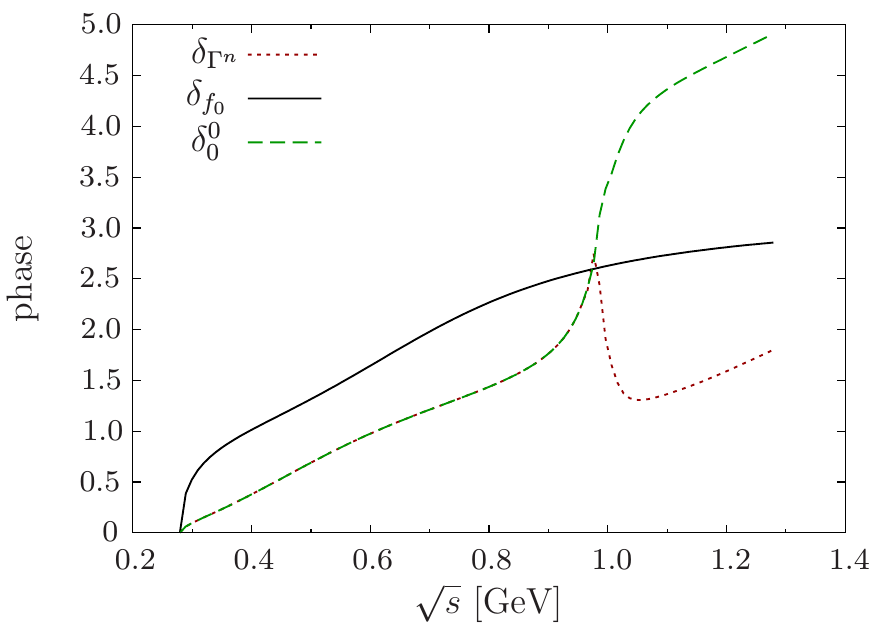
\includegraphics[width=\textwidth]{pipiPhaseReanalysis}}

\annot{11}{2.5}{\scriptsize LHCb fit}
\annot{12}{3.7}{\scriptsize {\color{ForestGreen}dispersive fit}}

}

\frame{
\frametitle{Collaboration on Hadronic Amplitudes}
\large
The \alert{need and desire} to improve collaboration between phenomenologists and experiments has been documented previously. \\For example: \vspace{3mm}
\begin{itemize}
\item ATHOS Whitepaper:\\ Analysis Tools for Next-Generation Hadron Spectroscopy Experiments\\ {\scriptsize[Acta Phys.~Polon.~B46,2(2015)257]}
\vspace{3mm}
\item INT Whitepaper: Issues and Opportunities in Exotic Hadrons\\
 \Arxiv{1511.06779}
\vspace{3mm}
\item EMMI Rapid Reaction Task Force: Resonances in QCD \\
{\scriptsize[Nucl.~Phys.~A948(2016)93]}
\end{itemize}

}

\frame{
\frametitle{Model Institutions}
\large
Independent bodies have been established for specific topics already
\begin{itemize}
\item \link{http://www.slac.stanford.edu/xorg/hfag/}{HFAG} - Heavy Flavour Averaging Group 
\item \link{https://jpac.jlab.org/}{JPAC} - Joint Physics Analysis Center
\item \link{http://cnr2.kent.edu/~manley/BRAG.html}{BRAG} - Baryon Resonance Analysis Group
\vspace{3mm}
\item \link{http://gwdac.phys.gwu.edu/}{INS Data Analysis Center}
\item \link{http://ckmfitter.in2p3.fr/}{CKM fitter} / \link{http://www.utfit.org/}{UTfit}
\end{itemize}
\vspace{5mm}
\alert{For amplitude analysis such an institution is missing in Europe}
}


\frame{
\frametitle{PHASE -- Panel on Hadronic Amplitudes}
\begin{center}
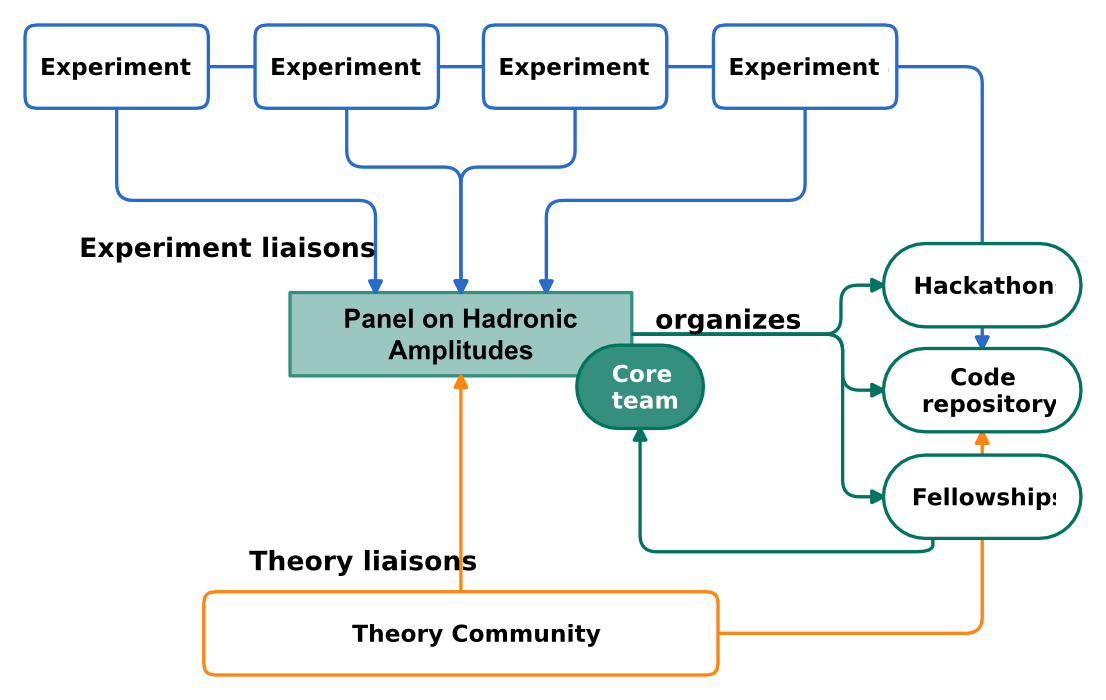
\includegraphics[width=0.8\textwidth]{PHASEstructure.png}
\end{center}

}


\frame{
\frametitle{Vision of the Initiative}
\begin{itemize}
\item Enable joint analyses of hadronic processes across multiple experiments and multiple data sets
\vspace{5mm}
\item Provide a forum and infrastructure for joint developments within the hadron physics community
\vspace{5mm}
\item Define best practices
\vspace{5mm}
\item Provide researchers with useful tools for data analysis
\end{itemize}
}

\frame{
\frametitle{Code-Repository as Center-Piece}
\large
\begin{itemize}
\item Analysis \alert{code is the essence} of amplitude analysis
\vspace{3mm}
\item Need a place to publish and discuss code between experimentalists and theorists
\vspace{3mm}
\item Focus on \alert{advanced models that cannot be produced by a single collaboration}
\vspace{3mm}
\item Workshops are great, but we need to walk the walk
\vspace{5mm}
\item GITLAB repository and collaboration platform\\
 {\small TBD: host at CERN (provide easy access to non-CRN users)}
\end{itemize}

}

\frame{
\frametitle{Role of the Panel}
\large
\vspace{5mm}
\begin{itemize}
\item Ensure the \alert{flow of information} 
\vspace{3mm}
\item \alert{Curate} the PHASE repository
\vspace{3mm}
\item Ensure \alert{open access} to the repository
\vspace{3mm}
\item Facilitating a fair scrutiny of the contributed models
\vspace{3mm}
\item Regular \alert{review article} on the state of art of amplitude analyses.
\vspace{3mm}
\item Draft joint funding applications for the PHASE project.
\end{itemize}

\mannot{9}{0.1}{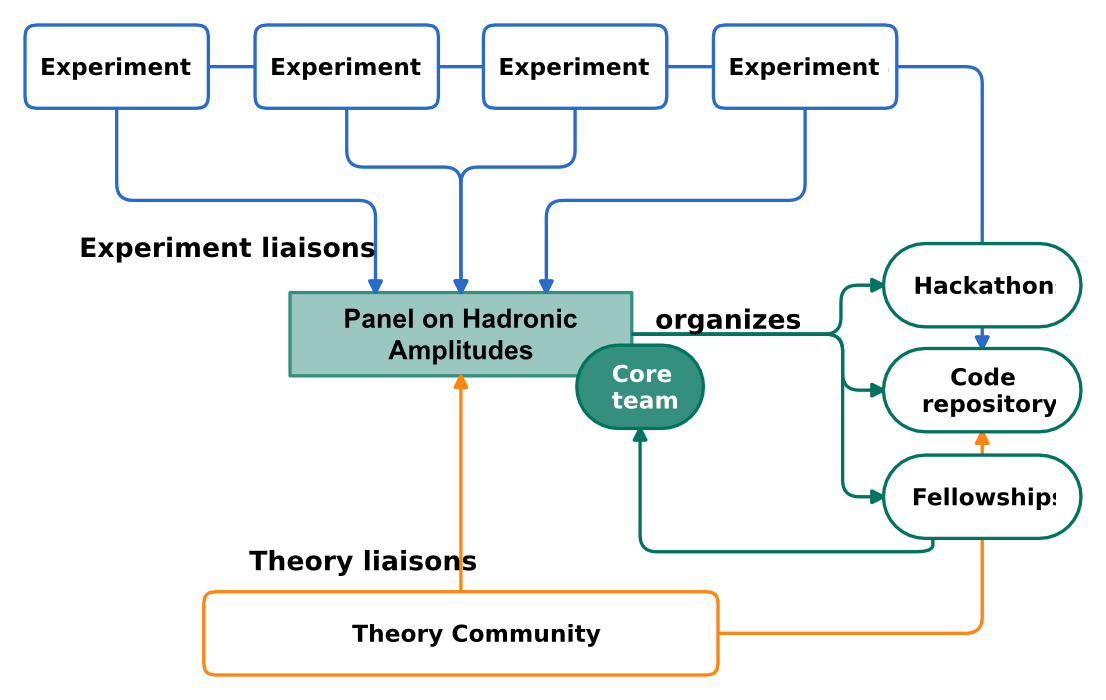
\includegraphics[width=\textwidth]{PHASEstructure.png}}


}





\frame{
\frametitle{Additional Activities}
\large
Things PHASE will do:
\vspace{3mm}
\begin{itemize}
\item Organize amplitude analysis \alert{hackathons}
\vspace{3mm}
\item Provide \alert{validation} of amplitude models
\vspace{3mm}
\item Community building
\vspace{3mm}
\item Advocate for \alert{Open-Data} initiatives
\vspace{3mm}
\item PHASE fellowships
\end{itemize}
}

\frame{
\frametitle{PHASE Proposal}
\large
\begin{itemize}
\item Initiated at 2016 MIAPP Workshop\\ Flavour Physics with High-Luminosity Experiments
\vspace{5mm}
\item \link{https://www.authorea.com/users/42472/articles/136761/_show_article}{PROPOSAL Document} {\scriptsize \url{https://www.authorea.com/users/42472/articles/136761/_show_article} }
\vspace{5mm}
\item Drafted by members of the following collaborations\\
\alert{LHCb, Belle II, BES III, COMPASS, PANDA, BaBar\\}
plus theory groups \alert{Juelich, Bonn, Madrid}\\
\vspace{5mm}
\item Will reach out to KLOE-2, CB-Elsa, CrystalBall@MaMi, SND, CMD-3, WASA, ALICE, FOPI
\end{itemize}

\annot{13}{2}{
\includegraphics[width=1cm]{lhcb-logo}}
\annot{14.2}{2}{
\includegraphics[width=1cm]{BES3_logo}}
\annot{13}{3.1}{
\includegraphics[width=1cm]{B-logo}}
\annot{14.2}{3}{
\includegraphics[width=1cm]{compass_logo}}
\annot{13}{4.2}{
\includegraphics[width=2.2cm]{Panda_Logo}}
\annot{13.2}{4.8}{
\includegraphics[width=2cm]{BABAR2}}

}

\frame{
\frametitle{Next Steps}
\Large
\begin{itemize}
\item Official email to be sent on 10th of February
\vspace{8mm}
\item Dedicated session on \alert{Monday 13th of April} at\\ ATHOS Workshop in Bad Honeff 
\begin{itemize}
\item Collect and discuss feedback
\item Start forming first panel
\end{itemize}
\end{itemize}
}



\frame{
\frametitle{How can LHCb take part?}
\Large
\begin{itemize}
\item Shape the initiative by giving \alert{feedback} on the PHASE proposal
\vspace{5mm}
\item Find \alert{Two Liaisons} to serve as panel members
\begin{itemize}
\item Until LHCB week?
\end{itemize}
\vspace{5mm}
\item Start discussion in AmAn-meeting and WGs, what topics/projects would be useful for us \\
$\rightarrow$ bring those into PHASE

\end{itemize}
}


\beginbackup

\frame{
\begin{center}
\Large Backup
\end{center}
}


\frame{
\frametitle{Repository Curation}
\large
\begin{center}
\begin{block}{Curation (wiktionary)}
\begin{itemize}
\item The act of curating, of \alert{organizing and maintaining} a collection of artworks or artifacts.
\vspace{3mm}
\item (archaic) The act of curing or healing.
\vspace{3mm}
\item (databases) The manual updating of information in a database.
\end{itemize}
\end{block}
\end{center}
}

\frame{
\frametitle{Tools which could live in the PHASE repo}
Adapted from [Acta Phys.~Polon.~B46,2(2015)257]
\vspace{3mm}
\begin{itemize}
\item \alert{Amplitude code}
\item MC generators
\item Data readers
\item Minimizers
\item Integrators
\item Plotters
\item Parallelization libraries
\item Exchange ideas (code snippets)
\item \alert{Ecosystem of coexisting, independent code}
\end{itemize}
}


%\frame{
%\tableofcontents
%}
\frame{
\frametitle{A Reference Implementation}
\large
\begin{itemize}
\item The purpose of the library is to implement the \alert{physics functions} needed for amplitude analysis.
\item While we will try to make it fast, optimization towards certain technologies is not the main focus of the effort.
\vspace{5mm}
\item It will become a \alert{reference implementation} 
\begin{itemize}
\item Analysers can use the library directly in their fitters
\item Comes with a \alert{test-suite} to compare custom implementations against
\end{itemize}
\item Working groups and reviewers will be able to request\\ \alert{consistency checks} against the reference library.
\vspace{5mm}
\item Goal: a \alert{consistent, tested and documented set of functions}\\ for all amplitude analyses in LHCb
\item Can be used to communicate our models to theorists
\end{itemize}
}



\frame{
\frametitle{Making Contributions to the PHASE repository}
\large
\begin{itemize}
\item The repository will be open
\item \alert{Everybody} can contribute
\item In practice: Any people developing models or doing analysis
\vspace{5mm}
\item Contributions are handled through a \alert{standard process} such as the \link{https://rfc.zeromq.org/spec:42/C4/}{C4 Collective Code Construction Contract}
\vspace{5mm}
\item PHASE panel members can contribute but their main job is to curate, i.e. set up and maintain the process
\end{itemize}
}

\frame{
\frametitle{Amplitude Analysis Hackathons}
\Large
\begin{itemize}
\item Get a group of experts together for 3 weeks
\item Concrete task to implement e.g. a certain amplitude model that is needed
\item Pay for accommodation during workshop
\item Results will be made public through PHASE servers
\end{itemize}
}


\backupend
\end{document}






